\documentclass[a0paper,portrait]{baposter}
\usepackage{wrapfig}
\usepackage{lmodern}
\usepackage[utf8]{inputenc} %unicode support
\usepackage[T1]{fontenc}
\usepackage{array}
\usepackage{multirow}
\usepackage{multicol}
\usepackage{amssymb}
\usepackage{amsmath}
\usepackage{amsfonts}
\selectcolormodel{cmyk}
\graphicspath{{figures/}} % Directory in which figures are stored
\usepackage{hyperref}
\newcommand{\compresslist}{\setlength{\itemsep}{0pt}\setlength{\parskip}{1pt}\setlength{\parsep}{0pt}}
\newenvironment{boenumerate}{\begin{enumerate}\renewcommand\labelenumi{\textbf\theenumi.}}{\end{enumerate}}

\begin{document}
	\definecolor{darkgreen}{cmyk}{0.8,0,0.8,0.45}
	\definecolor{lightgreen}{cmyk}{0.8,0,0.8,0.25}
	\begin{poster}
		{
			grid=false,
			headerborder=open, % Adds a border around the header of content boxes
			colspacing=1em, % Column spacing
			bgColorOne=white, % Background color for the gradient on the left side of the poster
			bgColorTwo=white, % Background color for the gradient on the right side of the poster
			borderColor=darkgreen, % Border color
			headerColorOne=lightgreen, % Background color for the header in the content boxes (left side)
			headerColorTwo=lightgreen, % Background color for the header in the content boxes (right side)
			headerFontColor=white, % Text color for the header text in the content boxes
			boxColorOne=white, % Background color of the content boxes
			textborder=rounded, %rectangle, % Format of the border around content boxes, can be: none, bars, coils, triangles, rectangle, rounded, roundedsmall, roundedright or faded
			eyecatcher=false, % Set to false for ignoring the left logo in the title and move the title left
			headerheight=0.11\textheight, % Height of the header
			headershape=rounded, % Specify the rounded corner in the content box headers, can be: rectangle, small-rounded, roundedright, roundedleft or rounded
			headershade=plain,
			headerfont=\Large\textsf, % Large, bold and sans serif font in the headers of content boxes
			%textfont={\setlength{\parindent}{1.5em}}, % Uncomment for paragraph indentation
			linewidth=2pt % Width of the border lines around content boxes
		}
		{}
		{
			{\small Projet de Fin d'Études 2022-2023}
			\sf\vspace{0.3em}\\
			\\\textsf
			{Navigation et contrôle multi-robots pour l'inspection acoustique de structures métallique}
		}
		{
			\sf\vspace{0.5em}\\
			Brandon ALVES
			\vspace{0.1em}\\
			\small{
				Département Informatique, INSA Lyon - CITI Lab. INSA - INRIA
				\vspace{0.2em}\\
				bdasilvaal@insa-lyon.fr
				\vspace{0.2em}\\
			}
		}
		{
			\hspace{0.5cm}
			
\includegraphics[height=1cm]{graphics/insa.jpg}
			\hspace{0.5cm}
			
\includegraphics[height=1cm]{graphics/citi.png}
		}
		\headerbox{1. Introduction}{name=intro,column=0,row=0,span=3}{
			L'inspection de structures métalliques est une tâche importante dans divers domaines tels que l'industrie, la construction et la maintenance.
			Elle vise à détecter les défauts et les anomalies, ce qui est crucial pour garantir la sécurité et la durabilité des structures.
			Les méthodes traditionnelles d'inspection manuelle sont souvent limitées en termes d'efficacité, de précision et de couverture.
			Nous proposons une approche basée sur la navigation et le contrôle multi-robots pour améliorer l'inspection acoustique des structures métalliques.
		}
		\headerbox{2. Problématique}{name=model,column=0,below=intro,span=1}{
			Nous cherchons à développer des algorithmes de navigation multi-robots, permettant une exploration coordonnée et une collecte de données acoustiques précises sur la structure métallique.
			Nous cherchons à :
			\begin{itemize}\compresslist
				\item Obtenir une couverture complète de la structure.
				\item Maximiser la précision de la cartographie des défauts sur la structure.
				\item Minimiser le temps nécessaire pour effectuer une inspection complète.
			\end{itemize}
		}
		\headerbox{3. Éléments techniques}{name=item,column=0,below=model,span=1}{
			Ces stratégies sont basées sur l'utilisation de robots de type "crawlers" équipés de capteurs tels qu'un capteur IMU, un capteur UGW pour l'émission et la réception d'ondes accoustiques et un capteur LIDAR. Les robots sont capables de se synchroniser pour se déplacer simultanément ou de manière alternée.

			\begin{center}
				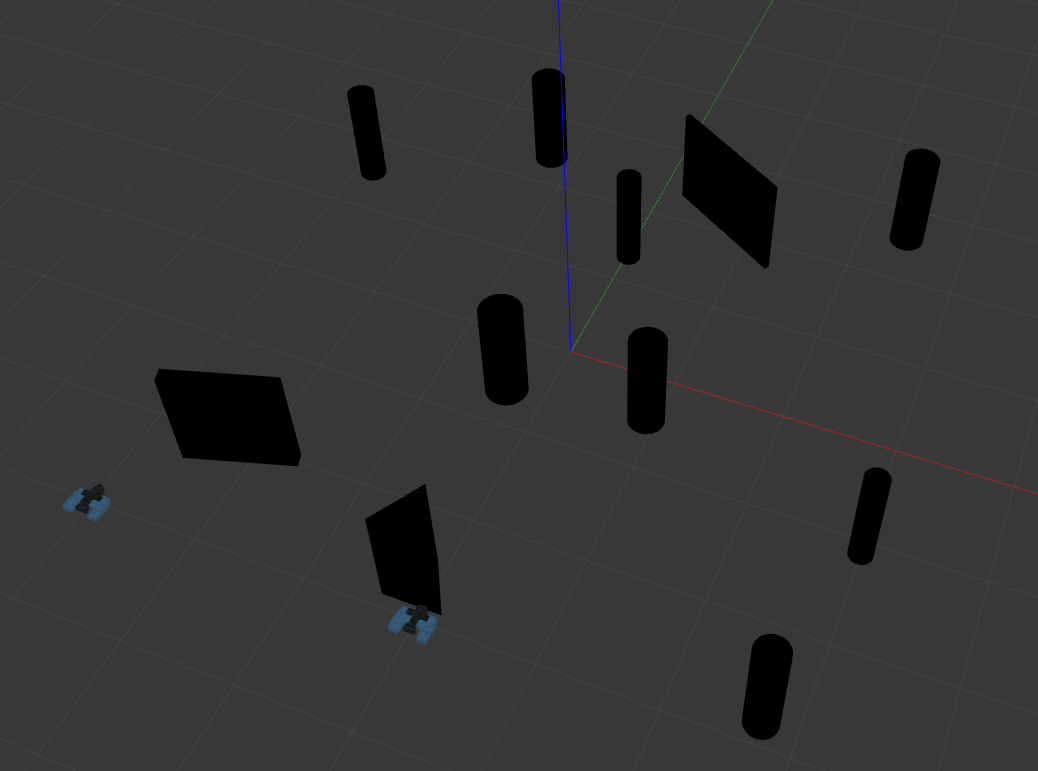
\includegraphics[height=80pt]{graphics/exemple_model.png}
				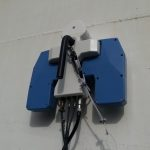
\includegraphics[height=80pt]{graphics/altiscan_closeup-150x150.jpg}
			\end{center}

			Nous avons utilisé Gazebo pour simuler l'environnement et les robots, et ROS pour la communication entre les robots et le contrôle de la simulation.
		}
		\headerbox{4. Proposition de solution}{name=prop,span=2,column=1,below=intro}{
			\begin{wrapfigure}{l}{0.4\textwidth}
				\vspace{-15pt}
				\begin{center}
					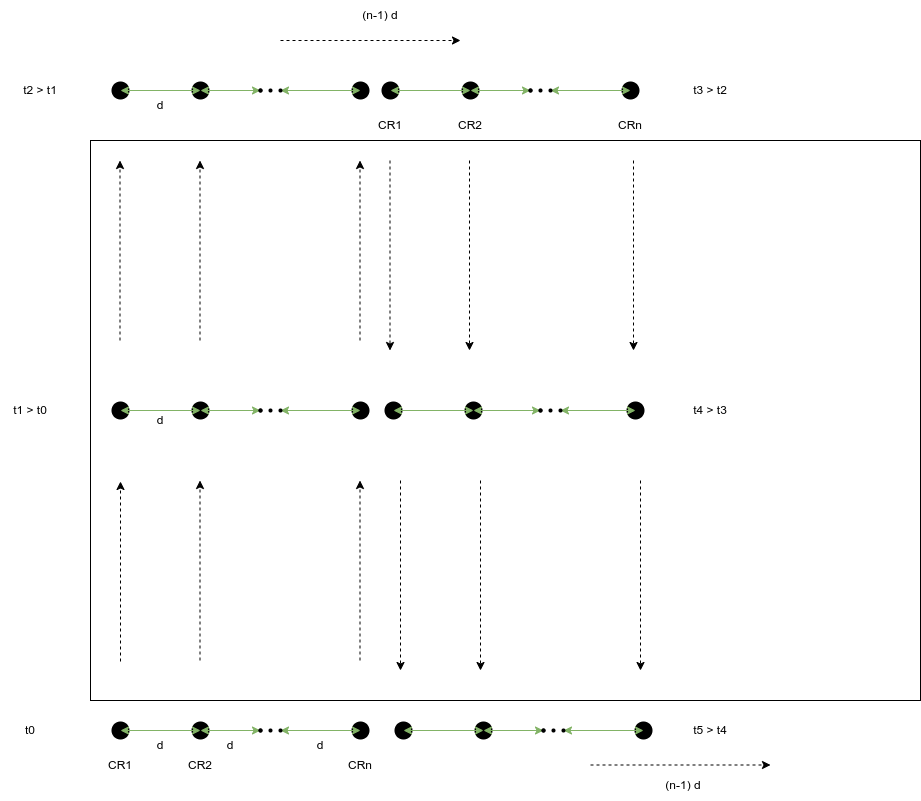
\includegraphics[width=0.9\linewidth]{graphics/peinture_au_rouleau.png}
					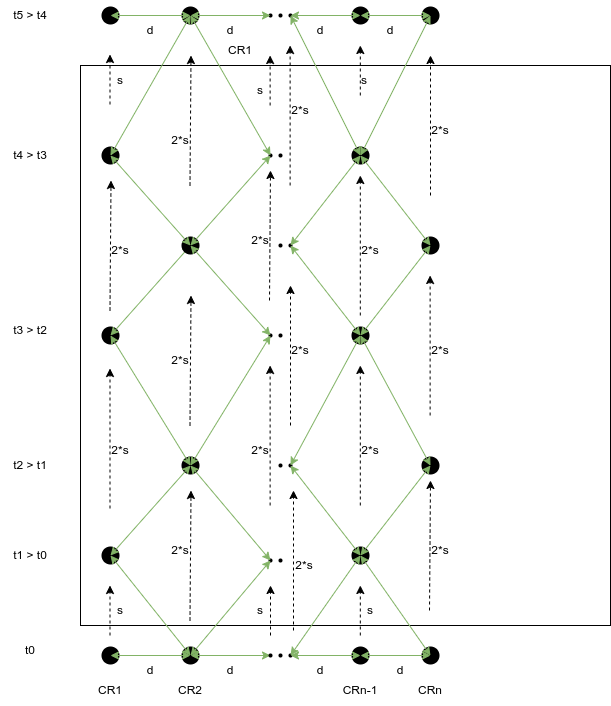
\includegraphics[width=0.9\linewidth]{graphics/ski_nordique_1.png}
				\end{center}
			\end{wrapfigure}

			Nous proposons trois stratégies de navigation multi-robots pour l'inspection acoustique de structures métalliques. Ces trois stratégies sont les suivantes :

			\begin{boenumerate}\compresslist
				\item Stratégie de navigation \textit{peinture au rouleau}
				\item Stratégie de navigation \textit{ski nordique}
				\item Stratégie de navigation \textit{investigation polygonale}
			\end{boenumerate}

			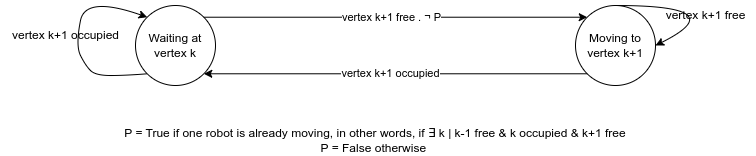
\includegraphics[width=0.95\linewidth]{graphics/automat_poly.png}

			Une grille d'occupation est utilisée pour modéliser l'environnement et obtenir en temps réel l'état de la surface métallique pendant l'inspection.
			Nous nous appuyons sur l'algorithme du tracé de segment de Bresenham~\cite{enwiki:1155124335} dans le processus de mise à jour de la grille d'occupation.
			\begin{center}
				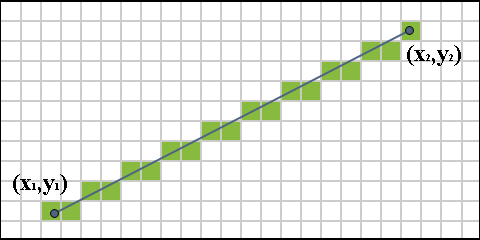
\includegraphics[width=0.45\linewidth]{graphics/Bresenham_line.png}
				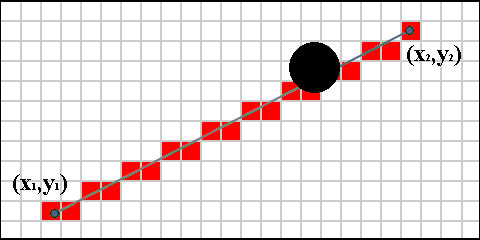
\includegraphics[width=0.45\linewidth]{graphics/Bresenham_line_2.png}
				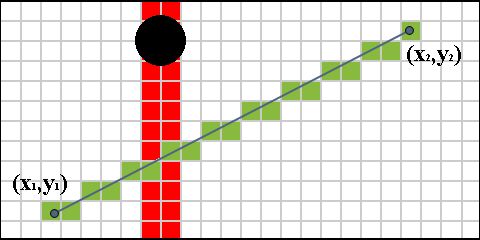
\includegraphics[width=0.45\linewidth]{graphics/Bresenham_line_3.png}
				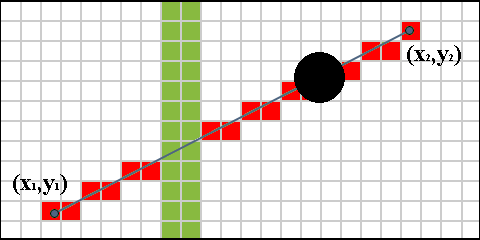
\includegraphics[width=0.45\linewidth]{graphics/Bresenham_line_4.png}
			\end{center}
		}
		\headerbox{5. Évaluation de la proposition}{name=eval,span=2,column=1,below=prop,above=bottom}{
			\begin{wrapfigure}[6]{r}{0.3\textwidth}
				\vspace{-15pt}
				\begin{center}
					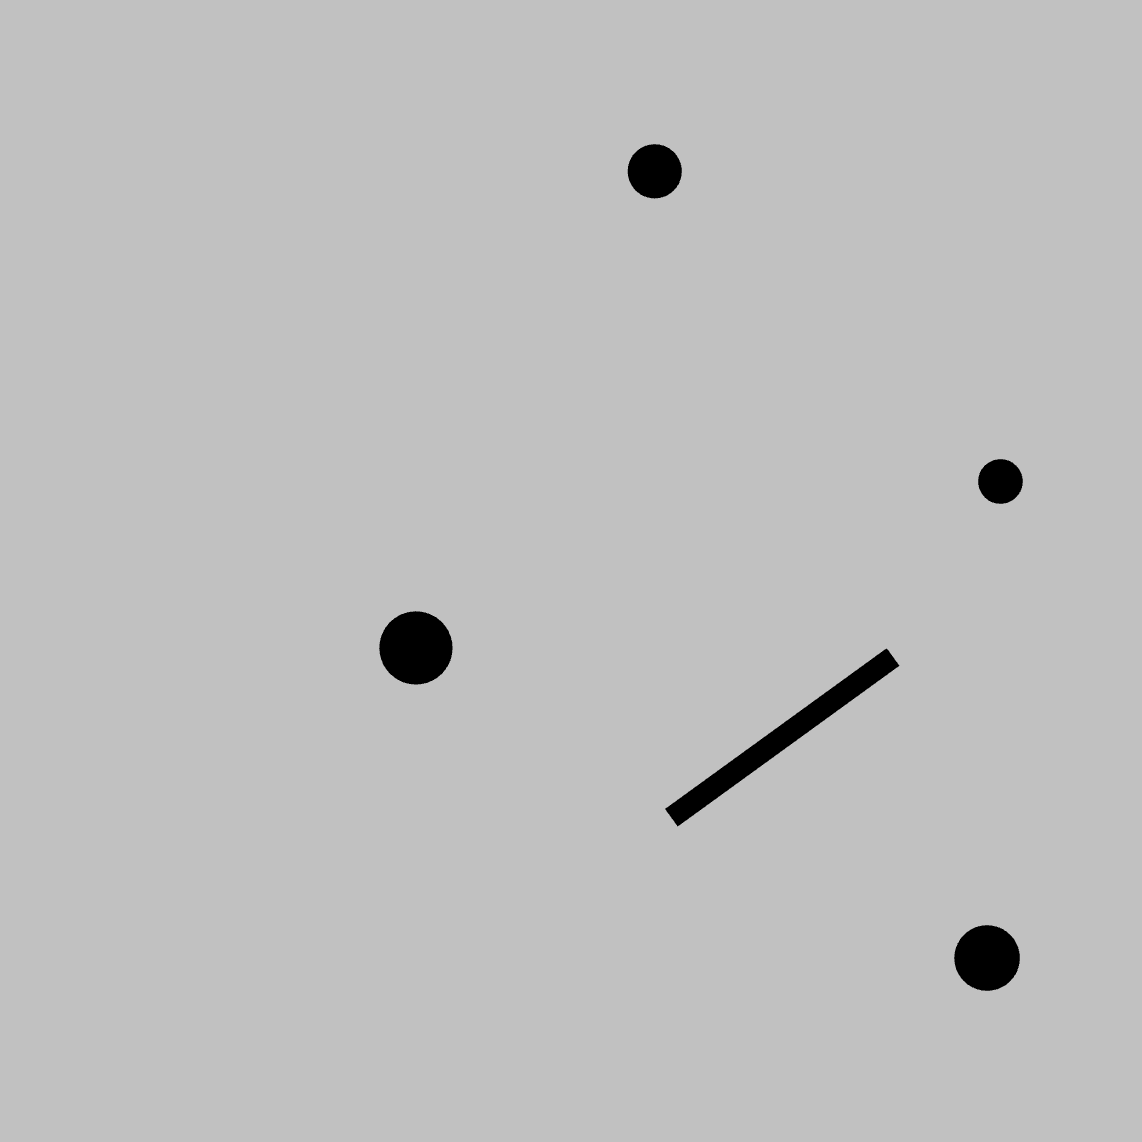
\includegraphics[width=0.3\linewidth]{graphics/test_model_05_1.png}
					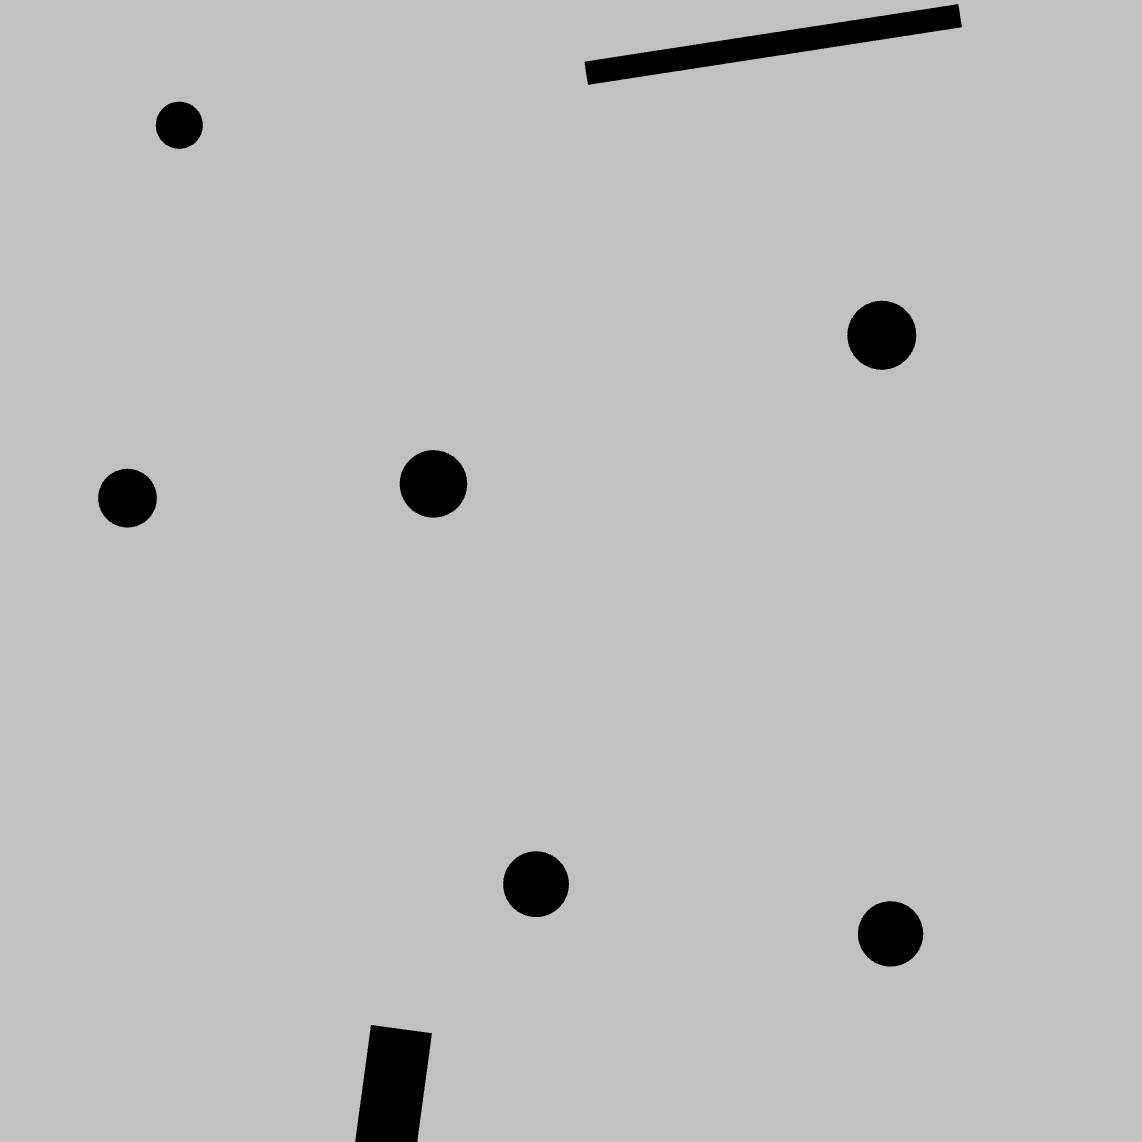
\includegraphics[width=0.3\linewidth]{graphics/test_model_08_1.png}
					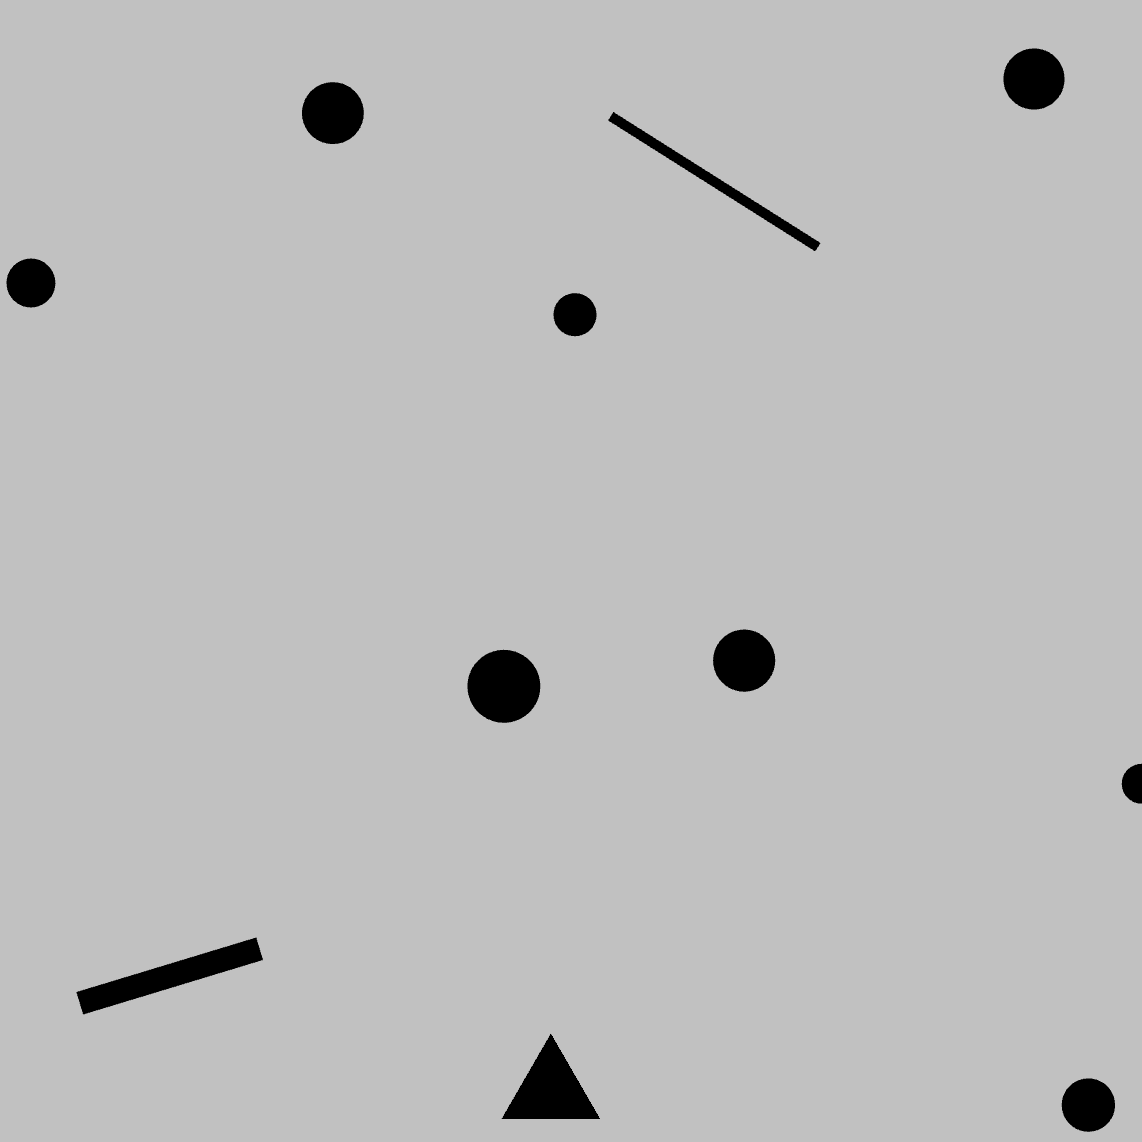
\includegraphics[width=0.3\linewidth]{graphics/test_model_11_1.png}
					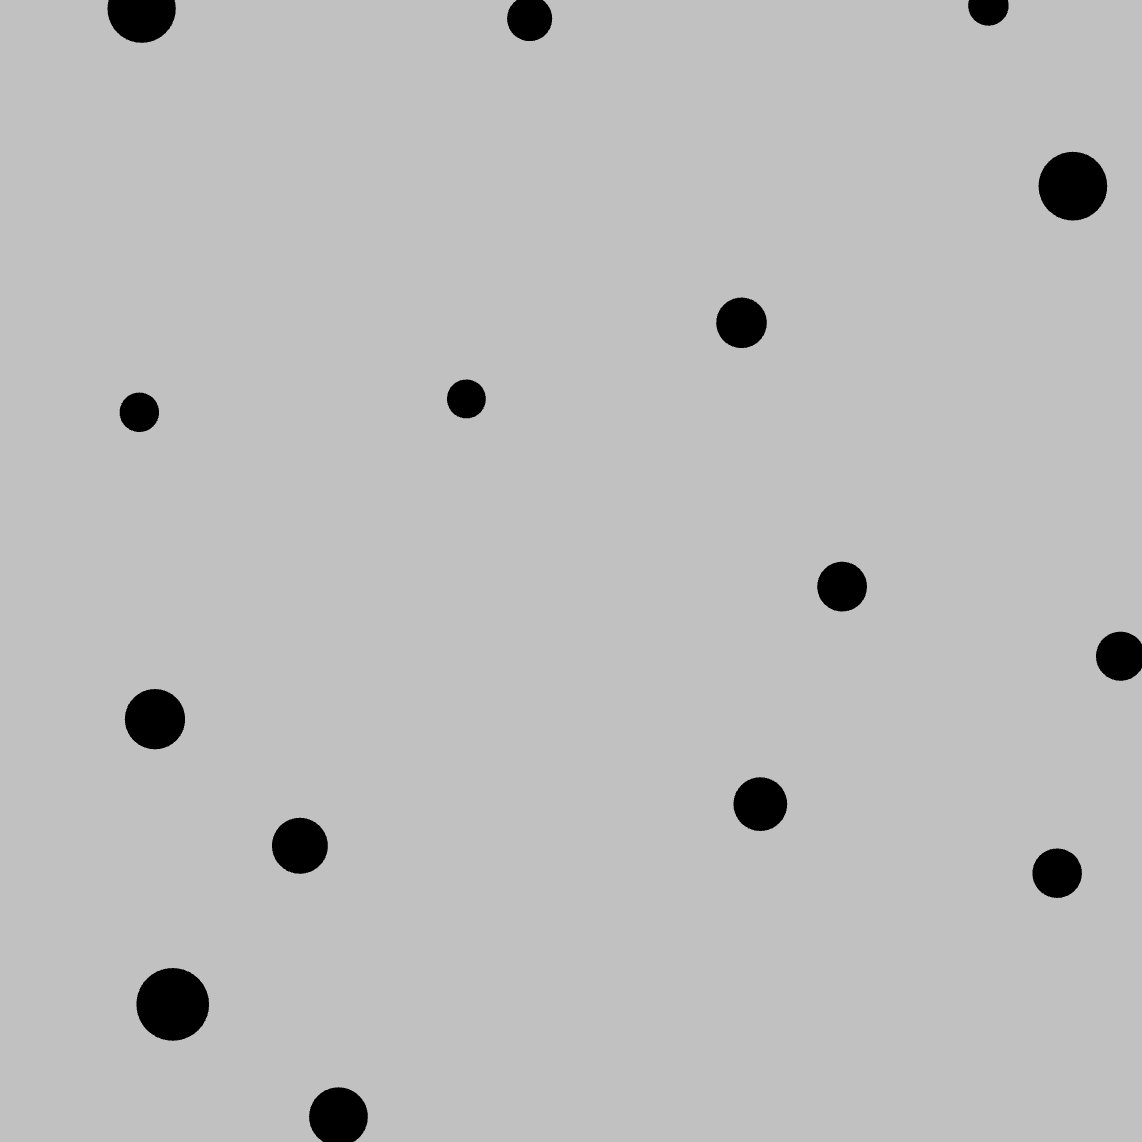
\includegraphics[width=0.3\linewidth]{graphics/test_model_15_1.png}
					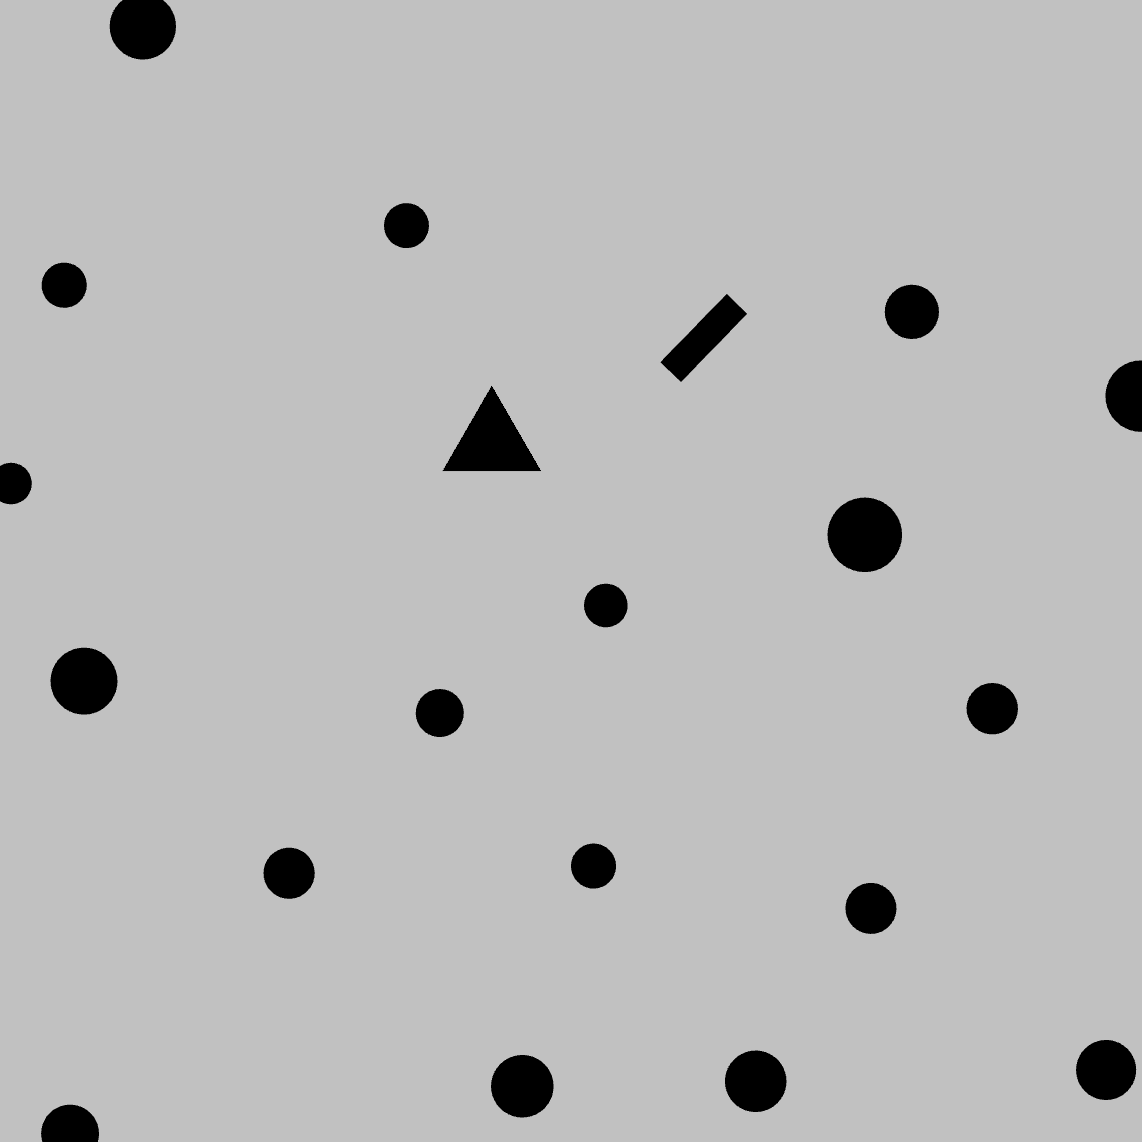
\includegraphics[width=0.3\linewidth]{graphics/test_model_20_1.png}
					
\includegraphics[width=0.3\linewidth]{graphics/test_model_30_1.png}
				\end{center}

				Score selon la métrique de Cohen~\cite{enwiki:1130024730} :
				\begin{equation*}
					\kappa = \frac{p_o - p_e}{1 - p_e}
				\end{equation*}

				Cartographies résultantes des zones de corrosion :
				\begin{center}
					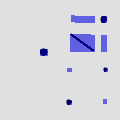
\includegraphics[width=0.3\linewidth]{graphics/both_example_par.png}
					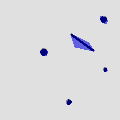
\includegraphics[width=0.3\linewidth]{graphics/both_example_sn.png}
					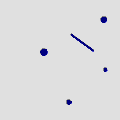
\includegraphics[width=0.3\linewidth]{graphics/both_example_ip.png}
				\end{center}
			\end{wrapfigure}

			Nous avons modélisé plusieurs cartes de tests qui modélisent une surface plane comportant différentes formes géométriques représentant les zones de corrosion à détecter et à localiser.
			La densité de corrosion varie en fonction des cartes.
			Nous avons évalué les performances des trois stratégies en termes de concordance avec la réalité et de temps d'inspection.

			\vspace{10pt}

			\begin{tabular}{|c|c|c|}
				\hline
				Stratégie & Paramètre & Valeurs \\
				\hline
				\multirow{2}{*}{\textit{peinture au rouleau}} & $n$ & 2 \\
				& $d$ & 1, 2, 3, 6 (mètres) \\
				\hline
				\multirow{3}{*}{\textit{ski nordique}} & $n$ & 2 \\
				& $d$ & 1, 2, 3, 6 (mètres) \\
				& $s$ & 1, 2, 3, 6 (mètres) \\
				\hline
				\multirow{5}{*}{\textit{investigation polygonale}} & stratégie initiale & \textit{peinture au rouleau} \\
				& $d$ & 1, 2, 3, 6 (mètres) \\
				& $n$ & 2 \\
				& $k$ & 1 \\
				& $p$ & 4, 6 \\
				\hline
			\end{tabular}

			\vspace{15pt}

			Nous avons également fait varier les paramètres des stratégies de navigation afin d'évaluer leur impact sur les performances de l'inspection.
			La stratégie \textit{investigation polygonale} est la plus performante en termes de concordance avec la réalité tandis que la stratégie \textit{peinture au rouleau} est la plus rapide.

			\vspace{5pt}

			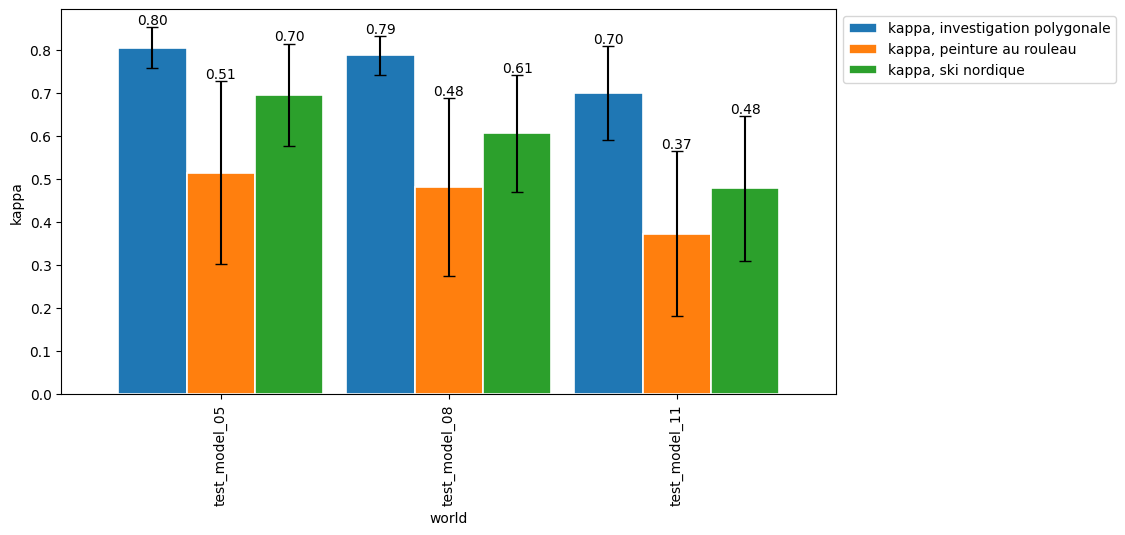
\includegraphics[width=0.5\linewidth]{graphics/investigation_polygonale-peinture_au_rouleau_ski_nordique-kappa_for_each_world_vs_investigation_polygonale-kappa_for_each_world.png}
			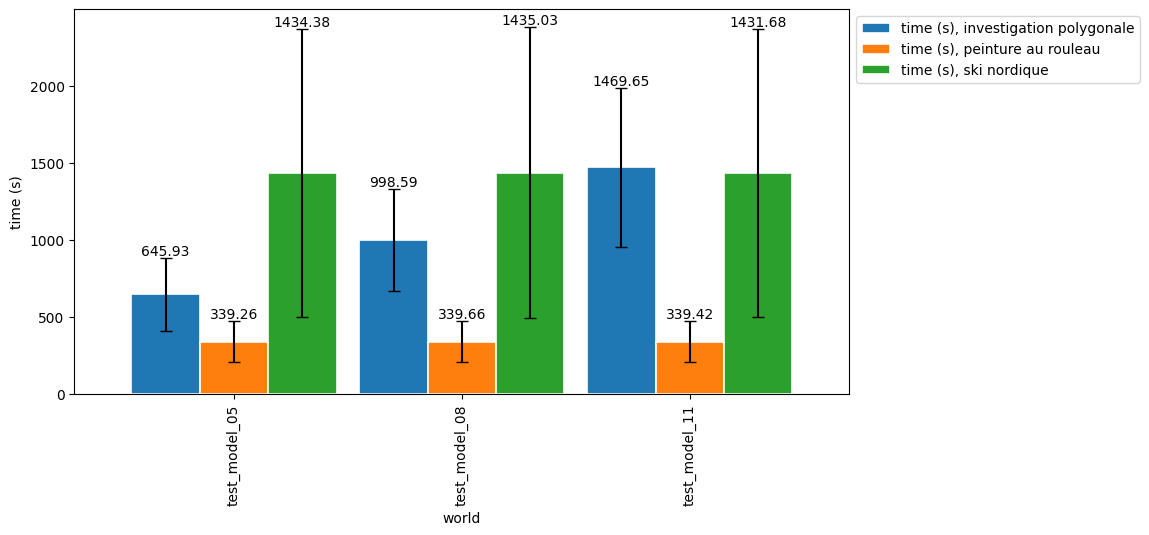
\includegraphics[width=0.5\linewidth]{graphics/investigation_polygonale-peinture_au_rouleau_ski_nordique-time_for_each_world_vs_investigation_polygonale-time_for_each_world.png}
		}
		\headerbox{6. Conclusions}{name=conclusion,column=0,below=item,span=1}{
			Nous avons développé et évalué trois stratégies de navigation pour la tomographie de structures métalliques.
			Pour ce faire, nous avons mis en place un environnement de simulation et un protocole d'évaluation avec métriques d'évaluation et scénarios de test.
			Nous avons également collecté des données de simulation et effectué des analyses statistiques.

			Il serait intéréssant, en termes de perspectives, d'implémenter ces stratégies sur des robots réels afin de les évaluer dans un environnement réel.
		}
		\headerbox{7. References}{name=references,column=0,span=1,below=conclusion,above=bottom}{
			\small
			\renewcommand{\section}[2]{\vskip 0.05em}
			% \nocite{*}
			\bibliographystyle{unsrt}
			\bibliography{RapportPFE}
		}
	\end{poster}
\end{document}

